We consider the class of strongly-scaled applications, and use $W$ to denote the size of an application workload~\cite{doe_ascr_exascale_2011}. The workload is split  arbitrarily into a set of $N$ tasks, whose synchronization is achieved using barriers. Assuming that each task is assigned to execute on a core at a maximum speed $\sigma=1$, the failure-free completion time of the application is $w = W/N$. 
Let $M_i$ denote the main process executing the $i^{th}$ task $T_i$, and $S_i$ its associated shadow.
When a failure occurs, the non-failing tasks continue executing until they reach the synchronization barrier. The tasks remain suspended until the shadow associated with the failing task reaches its synchronization barrier.


failure recovery is achieved.  To reduce time to recovery,  we run M shadows simulataneously with the main processes. 
%According to the computational model in Section~\ref{sec:com_model}, an application's workload is split into $M$ parallel tasks where each task is associated with a main process and a shadow.

 The execution of the application can be carried out by simultaneously running all main and shadow processes 
on %$2M$ cores, whereby the main processes execute at the maximum rate while the associated shadows execute at a fraction, $\sigma_s$, of the 
%maximum rate using DVFS. 
%To simultaneously run all the main and shadow processes,
%ne may choose to use $2M$ cores, with $M$ executing the main tasks at the maximum rate and $M$ \emph{lazily} executing the shadows at a fraction, $\sigma_s$, of the 
%maximum rate using DVFS.  
%An alternative method is to use 
$M+S$ cores, where $M$ is a multiple of $S$ and $M+S=N$, all executing at the maximum rate. $M$ of these cores are allocated to the main processes while the remaining $S$ cores are shared among their associated shadows. Based on this method, each main process is allocated one core, while $\alpha=M/S$ shadows are collocated on a single core. $\alpha$ is referred to as the main to shadow ratio.
For example, if $M=9$ and $S=3$, then the 9 shadows execute on 3 cores, with every $\alpha=3$ shadows executing on a core (Figure~\ref{fig:sc_mapping}).
%only $M+S$ cores can be used, whereby the main processes execute on the $M$ cores. And the $M$ shadows are divided into $S$ clusters with of $M/S$ shadows are colocated on a single core, operating at the maximum rate.
%where $M$ is a multiple of $S$, and collocate $M/S$ shadows on each of the $S$ cores, while executing all the cores at the maximum speed. 
%We use $\alpha$ to denote the main to shadow allocation ratio. %, and for simplicity, we assume the maximum execution rate of a core is 1. %Ignoring the overhead of context switching, the two alternatives lead to the same expected execution time, but different power and energy consumption. Specifically, the $2M$-cores scheme consumes more static but less dynamic power/energy than the $M+S$ cores alternative. The ratio between the system static and dynamic power consumption determines which alternative overall consumes less power/energy. 

%In the rest of the paper, we will focus on 
%shadow collocation as the meain the rest of our discussion 
%of the main ideas, concepts and system design. We will assume that all cores in the system execute at maximum speed, with every $\alpha=M/S$ shadows collocated on a core. 
%In HPC, throughput consideration requires that the rate of the main task, $\sigma_m$, and the shadow after failure, $\sigma_a$, be set to the maximum. The execution rate of the shadow before failure, $\sigma_b$, however, may still be used to manage the trade-offs between completion time and energy consumption. Smaller $\sigma_b$ corresponds to lazier shadowing of the main process. 
%In terms of execution rates, this can be expressed as $\sigma_m=\sigma_a=1$ and $\sigma_s \le 1$. 
  
Collocation of $\alpha$ shadows on a core has an important ramification with respect to the resilience of the system. Specifically, to speed up a shadow 
of a failed main to the maximum rate, all other collocated shadows must be terminated. Consequently, a second failure in any of the mains of the terminated shadows cannot be tolerated. In other words, the $M+S$ cores are grouped into $S$ sets, which we call \emph{shadowed sets}, each containing $\alpha+1$ cores with $\alpha$ mains executing on $\alpha$ cores (referred to as main cores) and their corresponding $\alpha$ shadows collocated on one core (referred to as shadow core). Each shadowed set can tolerate a failure in any of its cores, since failure of a main core would be recovered by the shadow core and failure of the shadow core will not affect any mains. After the first failure in a shadowed set, the set is called \emph{vulnerable} because it cannot tolerate another failure. %In the following subsection, we will discuss a rejuvenation scheme that deals with vulnerable shadowed sets.

\begin{figure}[!t]
	\begin{center}
		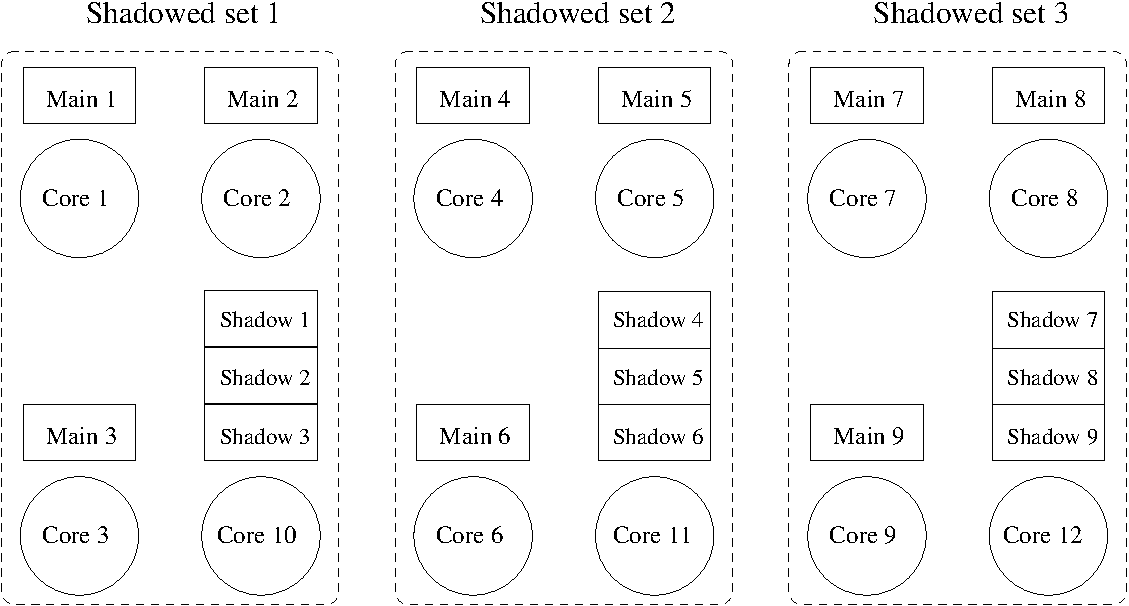
\includegraphics[width=\columnwidth]{Figures/sc_mapping.pdf}
	\end{center}
	\vskip -0.25in 
	\caption{An example of 3 shadowed sets with $\alpha=3$.}
	\label{fig:sc_mapping}
\end{figure}
